\documentclass[]{article}
\usepackage{lmodern}
\usepackage{amssymb,amsmath}
\usepackage{ifxetex,ifluatex}
\usepackage{fixltx2e} % provides \textsubscript
\ifnum 0\ifxetex 1\fi\ifluatex 1\fi=0 % if pdftex
  \usepackage[T1]{fontenc}
  \usepackage[utf8]{inputenc}
\else % if luatex or xelatex
  \ifxetex
    \usepackage{mathspec}
    \usepackage{xltxtra,xunicode}
  \else
    \usepackage{fontspec}
  \fi
  \defaultfontfeatures{Mapping=tex-text,Scale=MatchLowercase}
  \newcommand{\euro}{€}
\fi
% use upquote if available, for straight quotes in verbatim environments
\IfFileExists{upquote.sty}{\usepackage{upquote}}{}
% use microtype if available
\IfFileExists{microtype.sty}{%
\usepackage{microtype}
\UseMicrotypeSet[protrusion]{basicmath} % disable protrusion for tt fonts
}{}
\usepackage[margin=1in]{geometry}
\usepackage{color}
\usepackage{fancyvrb}
\newcommand{\VerbBar}{|}
\newcommand{\VERB}{\Verb[commandchars=\\\{\}]}
\DefineVerbatimEnvironment{Highlighting}{Verbatim}{commandchars=\\\{\}}
% Add ',fontsize=\small' for more characters per line
\usepackage{framed}
\definecolor{shadecolor}{RGB}{248,248,248}
\newenvironment{Shaded}{\begin{snugshade}}{\end{snugshade}}
\newcommand{\KeywordTok}[1]{\textcolor[rgb]{0.13,0.29,0.53}{\textbf{{#1}}}}
\newcommand{\DataTypeTok}[1]{\textcolor[rgb]{0.13,0.29,0.53}{{#1}}}
\newcommand{\DecValTok}[1]{\textcolor[rgb]{0.00,0.00,0.81}{{#1}}}
\newcommand{\BaseNTok}[1]{\textcolor[rgb]{0.00,0.00,0.81}{{#1}}}
\newcommand{\FloatTok}[1]{\textcolor[rgb]{0.00,0.00,0.81}{{#1}}}
\newcommand{\CharTok}[1]{\textcolor[rgb]{0.31,0.60,0.02}{{#1}}}
\newcommand{\StringTok}[1]{\textcolor[rgb]{0.31,0.60,0.02}{{#1}}}
\newcommand{\CommentTok}[1]{\textcolor[rgb]{0.56,0.35,0.01}{\textit{{#1}}}}
\newcommand{\OtherTok}[1]{\textcolor[rgb]{0.56,0.35,0.01}{{#1}}}
\newcommand{\AlertTok}[1]{\textcolor[rgb]{0.94,0.16,0.16}{{#1}}}
\newcommand{\FunctionTok}[1]{\textcolor[rgb]{0.00,0.00,0.00}{{#1}}}
\newcommand{\RegionMarkerTok}[1]{{#1}}
\newcommand{\ErrorTok}[1]{\textbf{{#1}}}
\newcommand{\NormalTok}[1]{{#1}}
\usepackage{graphicx}
\makeatletter
\def\maxwidth{\ifdim\Gin@nat@width>\linewidth\linewidth\else\Gin@nat@width\fi}
\def\maxheight{\ifdim\Gin@nat@height>\textheight\textheight\else\Gin@nat@height\fi}
\makeatother
% Scale images if necessary, so that they will not overflow the page
% margins by default, and it is still possible to overwrite the defaults
% using explicit options in \includegraphics[width, height, ...]{}
\setkeys{Gin}{width=\maxwidth,height=\maxheight,keepaspectratio}
\ifxetex
  \usepackage[setpagesize=false, % page size defined by xetex
              unicode=false, % unicode breaks when used with xetex
              xetex]{hyperref}
\else
  \usepackage[unicode=true]{hyperref}
\fi
\hypersetup{breaklinks=true,
            bookmarks=true,
            pdfauthor={Abbas Rizvi},
            pdftitle={STA 546 - Homework 1},
            colorlinks=true,
            citecolor=blue,
            urlcolor=blue,
            linkcolor=magenta,
            pdfborder={0 0 0}}
\urlstyle{same}  % don't use monospace font for urls
\setlength{\parindent}{0pt}
\setlength{\parskip}{6pt plus 2pt minus 1pt}
\setlength{\emergencystretch}{3em}  % prevent overfull lines
\setcounter{secnumdepth}{0}

%%% Use protect on footnotes to avoid problems with footnotes in titles
\let\rmarkdownfootnote\footnote%
\def\footnote{\protect\rmarkdownfootnote}

%%% Change title format to be more compact
\usepackage{titling}

% Create subtitle command for use in maketitle
\newcommand{\subtitle}[1]{
  \posttitle{
    \begin{center}\large#1\end{center}
    }
}

\setlength{\droptitle}{-2em}
  \title{STA 546 - Homework 1}
  \pretitle{\vspace{\droptitle}\centering\huge}
  \posttitle{\par}
  \author{Abbas Rizvi}
  \preauthor{\centering\large\emph}
  \postauthor{\par}
  \predate{\centering\large\emph}
  \postdate{\par}
  \date{February 24, 2016}



\begin{document}

\maketitle


\section{Problem 1}\label{problem-1}

The bodyfat dataset was considered. The bodyfat dataset consists of
bodyfat estimates by underwater weighing and various body circumference
measurements for 252 men.

\begin{Shaded}
\begin{Highlighting}[]
\KeywordTok{setwd}\NormalTok{(}\StringTok{"/Users/aarizvi/Google Drive/STA546/hw1/"}\NormalTok{)}
\KeywordTok{load}\NormalTok{(}\StringTok{"bodyfat.rdata"}\NormalTok{)}
\end{Highlighting}
\end{Shaded}

The task for this problem was to pre-process the data, such that
outliers, unusual distributions, and scaling issues are addressed. To
begin exploration of this dataset, the analysis began with looking at
the columns in order to address any scaling issues.

\begin{Shaded}
\begin{Highlighting}[]
\KeywordTok{head}\NormalTok{(bodyfat)}
\end{Highlighting}
\end{Shaded}

\begin{verbatim}
##   density bodyfat age weight height neck chest abdomen   hip thigh knee
## 1  1.0708    12.3  23 154.25  67.75 36.2  93.1    85.2  94.5  59.0 37.3
## 2  1.0853     6.1  22 173.25  72.25 38.5  93.6    83.0  98.7  58.7 37.3
## 3  1.0414    25.3  22 154.00  66.25 34.0  95.8    87.9  99.2  59.6 38.9
## 4  1.0751    10.4  26 184.75  72.25 37.4 101.8    86.4 101.2  60.1 37.3
## 5  1.0340    28.7  24 184.25  71.25 34.4  97.3   100.0 101.9  63.2 42.2
## 6  1.0502    20.9  24 210.25  74.75 39.0 104.5    94.4 107.8  66.0 42.0
##   ankle biceps forearm wrist
## 1  21.9   32.0    27.4  17.1
## 2  23.4   30.5    28.9  18.2
## 3  24.0   28.8    25.2  16.6
## 4  22.8   32.4    29.4  18.2
## 5  24.0   32.2    27.7  17.7
## 6  25.6   35.7    30.6  18.8
\end{verbatim}

It was quickly noticed that the units for columns weight
(\texttt{bodyfat\$weight}) and height (\texttt{bodyfat\$height}) are
measured in U.S. customary units and the remaining columns were measured
using SI units. This could be problematic when computing simple
calculations using the data, therefore \texttt{bodyfat\$weight} and
\texttt{bodyfat\$height} were converted into SI units.

\begin{Shaded}
\begin{Highlighting}[]
\NormalTok{bodyfat$weight <-}\StringTok{ }\KeywordTok{round}\NormalTok{((bodyfat$weight /}\StringTok{ }\FloatTok{2.2}\NormalTok{)*}\DecValTok{1000}\NormalTok{, }\DecValTok{2}\NormalTok{) }\CommentTok{#convert weight from lbs into grams}
\NormalTok{bodyfat$height <-}\StringTok{ }\KeywordTok{round}\NormalTok{(bodyfat$height *}\StringTok{ }\FloatTok{2.54}\NormalTok{, }\DecValTok{2}\NormalTok{) }\CommentTok{#convert height from inches into cm}
\end{Highlighting}
\end{Shaded}

Subsequently, the data was visualized using boxplots and histograms to
observe the distrubtions of the different column measurements and
identify any outliers (Figure 1).

\begin{Shaded}
\begin{Highlighting}[]
\CommentTok{#visualize boxplots for all columns}
\KeywordTok{par}\NormalTok{(}\DataTypeTok{mfrow =} \KeywordTok{c}\NormalTok{(}\DecValTok{3}\NormalTok{,}\DecValTok{5}\NormalTok{),}
          \DataTypeTok{oma =} \KeywordTok{c}\NormalTok{(}\DecValTok{5}\NormalTok{,}\DecValTok{4}\NormalTok{,}\DecValTok{0}\NormalTok{,}\DecValTok{0}\NormalTok{) +}\StringTok{ }\FloatTok{0.1}\NormalTok{,}
          \DataTypeTok{mar =} \KeywordTok{c}\NormalTok{(}\DecValTok{0}\NormalTok{,}\DecValTok{0}\NormalTok{,}\DecValTok{1}\NormalTok{,}\DecValTok{2}\NormalTok{) +}\StringTok{ }\FloatTok{0.1}\NormalTok{)}
\NormalTok{colnames <-}\StringTok{ }\KeywordTok{dimnames}\NormalTok{(bodyfat)[[}\DecValTok{2}\NormalTok{]]}
\NormalTok{for(i in }\DecValTok{1}\NormalTok{:}\KeywordTok{ncol}\NormalTok{(bodyfat))\{}
        \KeywordTok{boxplot}\NormalTok{(bodyfat[,i], }\DataTypeTok{main=}\NormalTok{colnames[i])}
\NormalTok{\}}
\end{Highlighting}
\end{Shaded}

\begin{figure}[htbp]
\centering
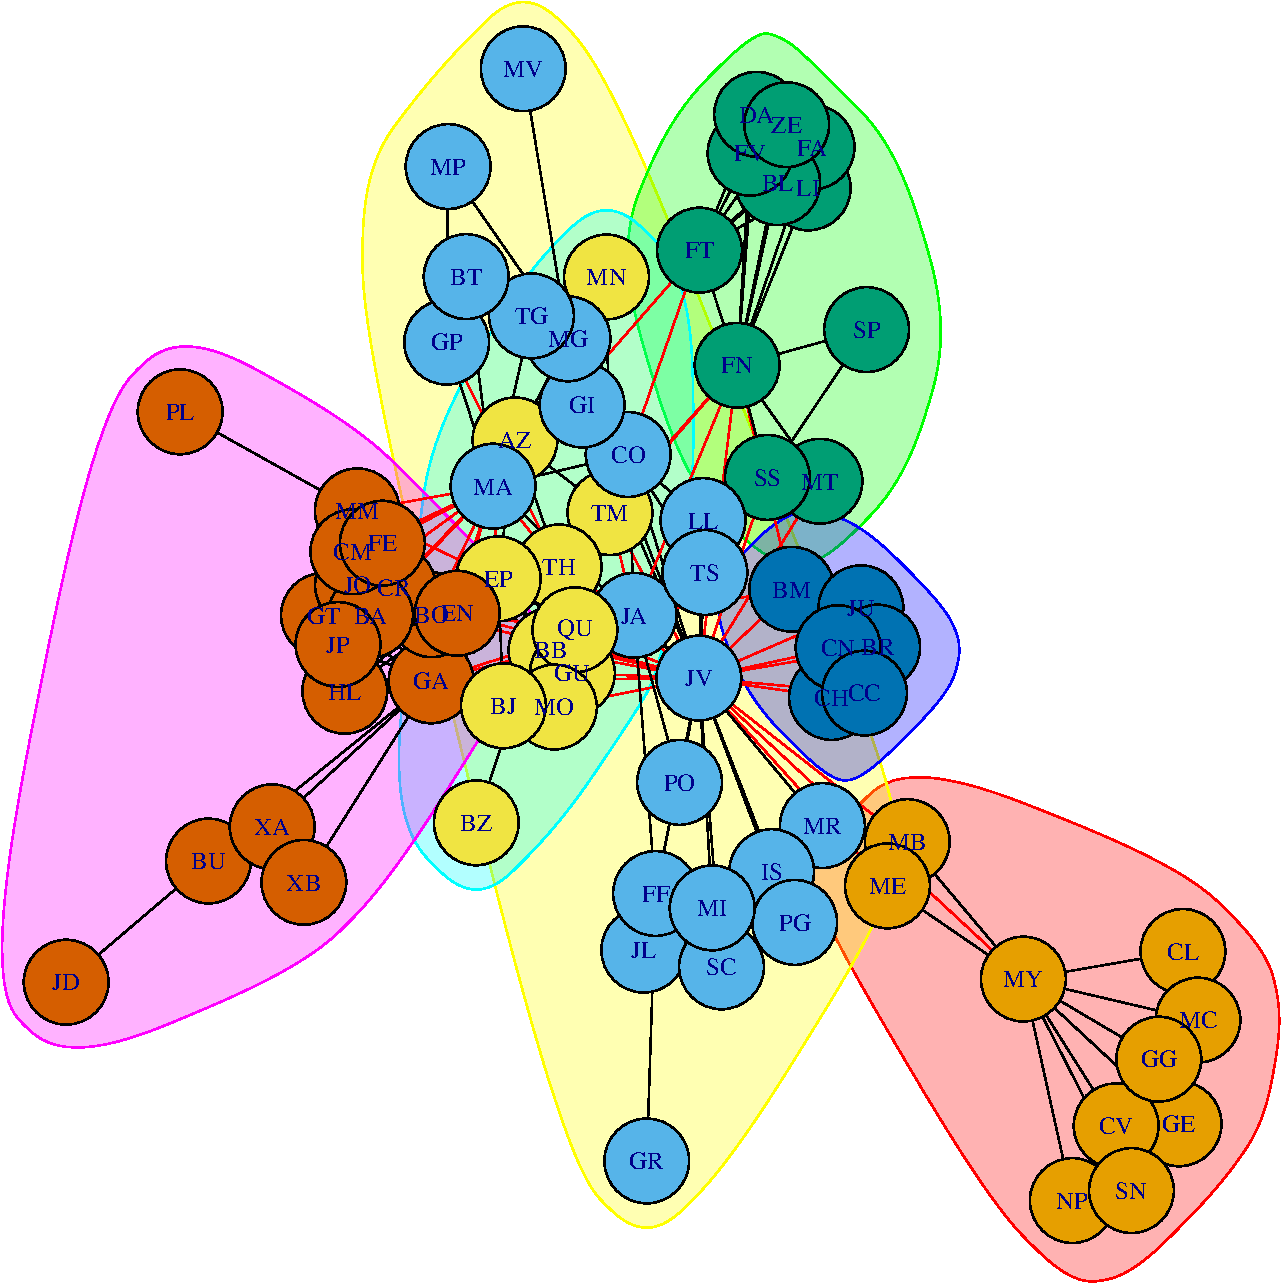
\includegraphics{RIZVI_HW1_STA546_files/figure-latex/unnamed-chunk-4-1.pdf}
\caption{Boxplots of bodyfat measurements}
\end{figure}

Outliers are noticeable in the most columns (Figure 1). Typically,
outliers are not removed, but for this exercise we shall remove outliers
in order to keep our dataset as simple as possible. But before removing
let's visualize this another way using histograms with overlayed density
plots of the different measurement groups (Figure 2).

\begin{Shaded}
\begin{Highlighting}[]
\CommentTok{#visualize histograms for all columns}
\KeywordTok{library}\NormalTok{(MASS)}
\KeywordTok{par}\NormalTok{(}\DataTypeTok{mfrow =} \KeywordTok{c}\NormalTok{(}\DecValTok{3}\NormalTok{,}\DecValTok{5}\NormalTok{),}
          \DataTypeTok{oma =} \KeywordTok{c}\NormalTok{(}\DecValTok{5}\NormalTok{,}\DecValTok{4}\NormalTok{,}\DecValTok{0}\NormalTok{,}\DecValTok{0}\NormalTok{) +}\StringTok{ }\FloatTok{0.1}\NormalTok{,}
          \DataTypeTok{mar =} \KeywordTok{c}\NormalTok{(}\DecValTok{3}\NormalTok{,}\DecValTok{3}\NormalTok{,}\DecValTok{1}\NormalTok{,}\DecValTok{1}\NormalTok{) +}\StringTok{ }\FloatTok{0.1}\NormalTok{)}
\NormalTok{for(i in }\DecValTok{1}\NormalTok{:}\KeywordTok{ncol}\NormalTok{(bodyfat))\{}
        \KeywordTok{truehist}\NormalTok{(bodyfat[,i], }\DataTypeTok{main=}\NormalTok{colnames[i], }\DataTypeTok{col=}\StringTok{"gray"}\NormalTok{, }\DataTypeTok{border=}\StringTok{"white"}\NormalTok{)}
             \NormalTok{d <-}\StringTok{ }\KeywordTok{density}\NormalTok{(bodyfat[,i])}
             \KeywordTok{lines}\NormalTok{(d, }\DataTypeTok{col=}\StringTok{"red"}\NormalTok{)}
\NormalTok{\}}
\end{Highlighting}
\end{Shaded}

\begin{figure}[htbp]
\centering
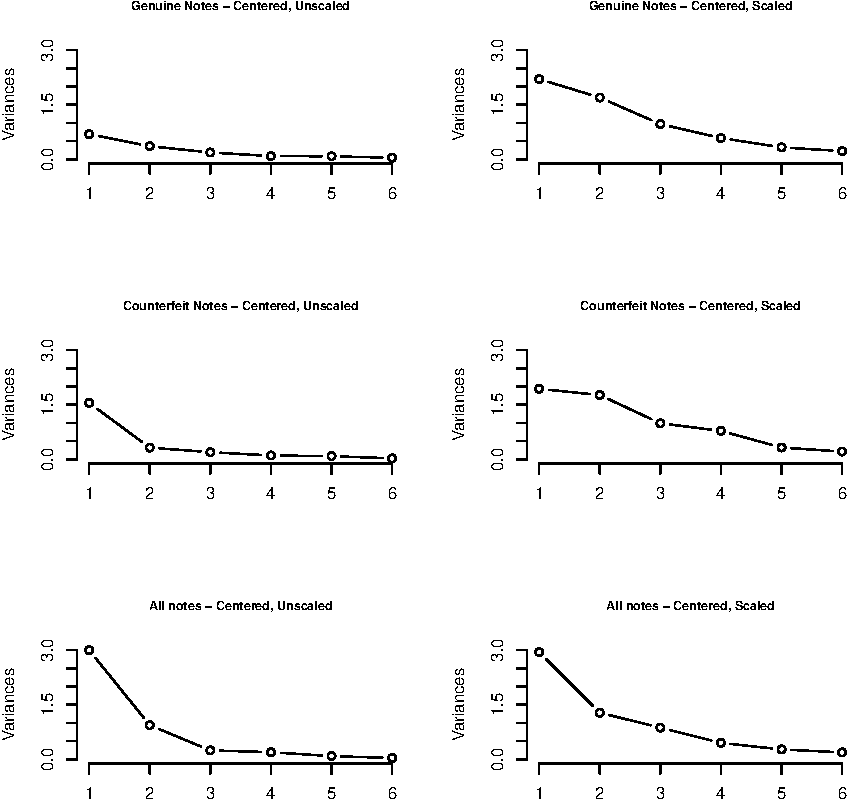
\includegraphics{RIZVI_HW1_STA546_files/figure-latex/unnamed-chunk-5-1.pdf}
\caption{Histograms of bodyfat measurements}
\end{figure}

The distributions all look approximately normal, however, there are some
with some noticeable tails, and that is due to the outliers. We will now
remove the outliers.

\begin{Shaded}
\begin{Highlighting}[]
\CommentTok{#now its time to remove outliers}
\NormalTok{indices <-}\StringTok{ }\KeywordTok{list}\NormalTok{()}
\NormalTok{for(i in }\DecValTok{1}\NormalTok{:}\KeywordTok{ncol}\NormalTok{(bodyfat))\{}
        \NormalTok{indices[[i]] <-}\StringTok{ }\KeywordTok{which}\NormalTok{(!bodyfat[,i] %in%}\StringTok{ }\KeywordTok{boxplot.stats}\NormalTok{(bodyfat[,i])$out ==}\StringTok{ 'FALSE'}\NormalTok{)      }
\NormalTok{\}}
\NormalTok{outlier.indices <-}\StringTok{ }\KeywordTok{unique}\NormalTok{(}\KeywordTok{unlist}\NormalTok{(indices))}
\NormalTok{bodyfat.clean <-}\StringTok{ }\NormalTok{bodyfat[-}\KeywordTok{c}\NormalTok{(outlier.indices),]}
\end{Highlighting}
\end{Shaded}

After dropping the row indices with outliers, the dataset has been
reduced to 235 observations from 252 observations. This data set has now
been pre-processed and saved as \texttt{clean\_data.RData} and can be
found in the attachment with the report.

The data was visualized again to see how the distributions changed after
removal of outliers (Figure 3).

\begin{Shaded}
\begin{Highlighting}[]
\CommentTok{#take a look at histograms/boxplots again}
\KeywordTok{par}\NormalTok{(}\DataTypeTok{mfrow =} \KeywordTok{c}\NormalTok{(}\DecValTok{3}\NormalTok{,}\DecValTok{5}\NormalTok{),}
          \DataTypeTok{oma =} \KeywordTok{c}\NormalTok{(}\DecValTok{5}\NormalTok{,}\DecValTok{4}\NormalTok{,}\DecValTok{0}\NormalTok{,}\DecValTok{0}\NormalTok{) +}\StringTok{ }\FloatTok{0.1}\NormalTok{,}
          \DataTypeTok{mar =} \KeywordTok{c}\NormalTok{(}\DecValTok{3}\NormalTok{,}\DecValTok{3}\NormalTok{,}\DecValTok{1}\NormalTok{,}\DecValTok{1}\NormalTok{) +}\StringTok{ }\FloatTok{0.1}\NormalTok{)}
\NormalTok{for(i in }\DecValTok{1}\NormalTok{:}\KeywordTok{ncol}\NormalTok{(bodyfat.clean))\{}
        \KeywordTok{truehist}\NormalTok{(bodyfat.clean[,i], }\DataTypeTok{main=}\NormalTok{colnames[i], }\DataTypeTok{col=}\StringTok{"gray"}\NormalTok{, }\DataTypeTok{border=}\StringTok{"white"}\NormalTok{)}
        \NormalTok{d <-}\StringTok{ }\KeywordTok{density}\NormalTok{(bodyfat.clean[,i])}
        \KeywordTok{lines}\NormalTok{(d, }\DataTypeTok{col=}\StringTok{"red"}\NormalTok{)}
\NormalTok{\}}
\end{Highlighting}
\end{Shaded}

\begin{figure}[htbp]
\centering
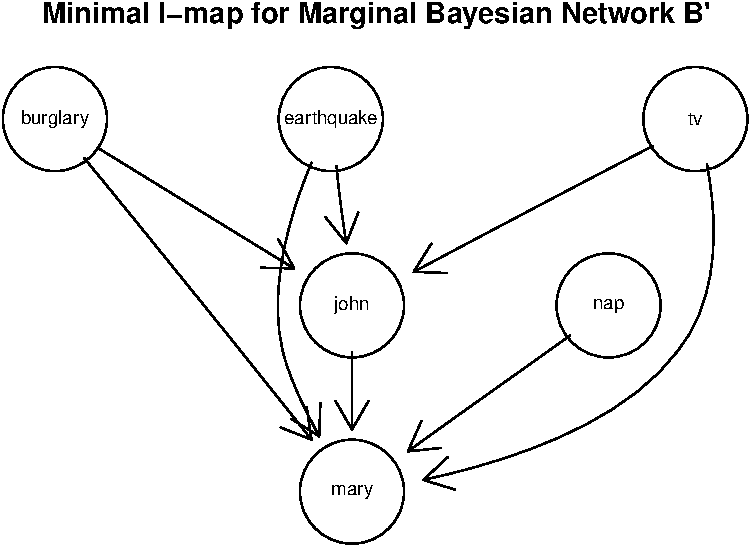
\includegraphics{RIZVI_HW1_STA546_files/figure-latex/unnamed-chunk-7-1.pdf}
\caption{Histograms with outliers removed}
\end{figure}

The histograms reveal that the outlier excluded data distributions
appear to be closer to `normal'.

\section{Problem 2}\label{problem-2}

This problem was adopted from
\href{http://infolab.stanford.edu/~ullman/mmds/ch9.pdf}{Chapter 9 -
Exercise 9.3.1}. We want to measure the similarity of users or items
from their rows or columns in a utility matrix. In order to measure the
similarity of two documents (or in this case, user's reviewing movies),
jaccard and cosine distances can be used.

The jaccard index is defined as the size of the intersections divided by
the size of the union between samples and the jaccard distance (which
measures the dissimilarity) is defined as 1-jaccard index. The following
function was written to represent the jaccard distance:

\begin{Shaded}
\begin{Highlighting}[]
\NormalTok{jaccard <-}\StringTok{ }\NormalTok{function(a, b)\{ }
        \NormalTok{int <-}\StringTok{ }\KeywordTok{sum}\NormalTok{(a[a==b])}
        \NormalTok{union <-}\StringTok{ }\KeywordTok{sum}\NormalTok{(a+b)-int }
        \KeywordTok{round}\NormalTok{(}\DecValTok{1}\NormalTok{-(int/union), }\DecValTok{4}\NormalTok{)}
\NormalTok{\}}
\end{Highlighting}
\end{Shaded}

The cosine similarity is a measure of similarity between two vectors of
an inner product space such that it measures the cosine of the angle
between the two vectors. Cosine simlarity is reprsented by:

\[similarity = cos(\theta) = \frac{\sum^{n}_{i=1}A_{i}B_{i}}{\sqrt{\sum^{n}_{i=1}A^{2}_{i}}\sqrt{\sum^{n}_{i=1}B^{2}_{i}}} \],
where \(A_{i}\) and \(B_{i}\) are componets of vector A and B

Cosine distance is 1-cosine similarity.

The following function was written for cosine dissimilarity:

\begin{Shaded}
\begin{Highlighting}[]
\NormalTok{cosine <-}\StringTok{ }\NormalTok{function(a, b)\{}
        \NormalTok{AB <-}\StringTok{ }\NormalTok{a*b}
        \NormalTok{AB <-}\StringTok{ }\KeywordTok{sum}\NormalTok{(AB)}
        \NormalTok{AA <-}\StringTok{ }\NormalTok{a^}\DecValTok{2}
        \NormalTok{AA <-}\StringTok{ }\KeywordTok{sum}\NormalTok{(AA)}
        \NormalTok{BB <-}\StringTok{ }\NormalTok{b^}\DecValTok{2}
        \NormalTok{BB <-}\StringTok{ }\KeywordTok{sum}\NormalTok{(BB)}
        \DecValTok{1}\NormalTok{-}\KeywordTok{round}\NormalTok{(AB/(}\KeywordTok{sqrt}\NormalTok{(AA)*}\KeywordTok{sqrt}\NormalTok{(BB)), }\DecValTok{4}\NormalTok{)}
\NormalTok{\}}
\end{Highlighting}
\end{Shaded}

\subsection{2.1}\label{section}

The utility matrix (\texttt{mat}) in Table 1 was considered.

\begin{Shaded}
\begin{Highlighting}[]
\KeywordTok{require}\NormalTok{(xtable)}
\NormalTok{mat <-}\StringTok{ }\KeywordTok{data.frame}\NormalTok{(}\KeywordTok{rbind}\NormalTok{(}\KeywordTok{c}\NormalTok{(}\DecValTok{4}\NormalTok{, }\DecValTok{5}\NormalTok{, }\DecValTok{0}\NormalTok{, }\DecValTok{5}\NormalTok{, }\DecValTok{1}\NormalTok{, }\DecValTok{0}\NormalTok{, }\DecValTok{3}\NormalTok{, }\DecValTok{2}\NormalTok{),}
                 \KeywordTok{c}\NormalTok{(}\DecValTok{0}\NormalTok{, }\DecValTok{3}\NormalTok{, }\DecValTok{4}\NormalTok{, }\DecValTok{3}\NormalTok{, }\DecValTok{1}\NormalTok{, }\DecValTok{2}\NormalTok{, }\DecValTok{1}\NormalTok{, }\DecValTok{0}\NormalTok{),}
                 \KeywordTok{c}\NormalTok{(}\DecValTok{2}\NormalTok{, }\DecValTok{0}\NormalTok{, }\DecValTok{1}\NormalTok{, }\DecValTok{3}\NormalTok{, }\DecValTok{0}\NormalTok{, }\DecValTok{4}\NormalTok{, }\DecValTok{5}\NormalTok{, }\DecValTok{3}\NormalTok{)))}
\KeywordTok{colnames}\NormalTok{(mat) <-}\StringTok{ }\KeywordTok{c}\NormalTok{(letters[}\DecValTok{1}\NormalTok{:}\DecValTok{8}\NormalTok{])}
\KeywordTok{rownames}\NormalTok{(mat) <-}\StringTok{ }\KeywordTok{c}\NormalTok{(}\StringTok{"1"}\NormalTok{, }\StringTok{"2"}\NormalTok{, }\StringTok{"3"}\NormalTok{)}
\NormalTok{xmat <-}\StringTok{ }\KeywordTok{xtable}\NormalTok{(mat, }
               \DataTypeTok{caption=}\StringTok{"Utility Matrix Adopted from 'Ch9 Recommendation Systems'"}\NormalTok{,}
               \DataTypeTok{digits=}\DecValTok{1}\NormalTok{)}
\KeywordTok{print.xtable}\NormalTok{(xmat, }\DataTypeTok{comment=}\OtherTok{FALSE}\NormalTok{)}
\end{Highlighting}
\end{Shaded}

\begin{table}[ht]
\centering
\begin{tabular}{rrrrrrrrr}
  \hline
 & a & b & c & d & e & f & g & h \\ 
  \hline
1 & 4.0 & 5.0 & 0.0 & 5.0 & 1.0 & 0.0 & 3.0 & 2.0 \\ 
  2 & 0.0 & 3.0 & 4.0 & 3.0 & 1.0 & 2.0 & 1.0 & 0.0 \\ 
  3 & 2.0 & 0.0 & 1.0 & 3.0 & 0.0 & 4.0 & 5.0 & 3.0 \\ 
   \hline
\end{tabular}
\caption{Utility Matrix Adopted from 'Ch9 Recommendation Systems'} 
\end{table}

The rows in table 1 are individual users and the columns are variables
for movies. The utility matrix (Table 1) was converted as Boolean under
the conditions that any values \textgreater{} 0 were converted as
\texttt{TRUE} and any values \textless{} 0 were converted to
\texttt{FALSE}.

\begin{Shaded}
\begin{Highlighting}[]
\NormalTok{## treat the utility matrix as boolean}
\NormalTok{boolean.mat <-}\StringTok{ }\KeywordTok{rbind}\NormalTok{(}\KeywordTok{c}\NormalTok{(}\OtherTok{TRUE}\NormalTok{, }\OtherTok{TRUE}\NormalTok{, }\OtherTok{FALSE}\NormalTok{, }\OtherTok{TRUE}\NormalTok{, }\OtherTok{TRUE}\NormalTok{, }\OtherTok{FALSE}\NormalTok{, }\OtherTok{TRUE}\NormalTok{, }\OtherTok{TRUE}\NormalTok{),}
                  \KeywordTok{c}\NormalTok{(}\OtherTok{FALSE}\NormalTok{, }\OtherTok{TRUE}\NormalTok{, }\OtherTok{TRUE}\NormalTok{, }\OtherTok{TRUE}\NormalTok{, }\OtherTok{TRUE}\NormalTok{, }\OtherTok{TRUE}\NormalTok{, }\OtherTok{TRUE}\NormalTok{, }\OtherTok{FALSE}\NormalTok{),}
                  \KeywordTok{c}\NormalTok{(}\OtherTok{TRUE}\NormalTok{, }\OtherTok{FALSE}\NormalTok{, }\OtherTok{TRUE}\NormalTok{, }\OtherTok{TRUE}\NormalTok{, }\OtherTok{FALSE}\NormalTok{, }\OtherTok{TRUE}\NormalTok{, }\OtherTok{TRUE}\NormalTok{, }\OtherTok{TRUE}\NormalTok{))}
\end{Highlighting}
\end{Shaded}

The Jaccard distance between users was computed for the
Boolean-converted utility matrix. This Boolean matrix essentially means
that if there was a rating reported by a user, they are considered
\texttt{TRUE} and if they didn't have a rating for the movies, they were
considered \texttt{FALSE}.

\begin{Shaded}
\begin{Highlighting}[]
\NormalTok{## compute Jaccard distance between users}
\NormalTok{User1vUser2.bool <-}\StringTok{ }\KeywordTok{jaccard}\NormalTok{(boolean.mat[}\DecValTok{1}\NormalTok{,], boolean.mat[}\DecValTok{2}\NormalTok{,])}
\NormalTok{User1vUser3.bool <-}\StringTok{ }\KeywordTok{jaccard}\NormalTok{(boolean.mat[}\DecValTok{1}\NormalTok{,], boolean.mat[}\DecValTok{3}\NormalTok{,])}
\NormalTok{User2vUser3.bool <-}\StringTok{ }\KeywordTok{jaccard}\NormalTok{(boolean.mat[}\DecValTok{2}\NormalTok{,], boolean.mat[}\DecValTok{3}\NormalTok{,])}
\KeywordTok{message}\NormalTok{(}\KeywordTok{paste0}\NormalTok{(}\StringTok{"Jaccard Distance between User 1 and 2 is: "}\NormalTok{, User1vUser2.bool, }\StringTok{"}\CharTok{\textbackslash{}n}\StringTok{"}\NormalTok{,}
               \StringTok{"Jaccard Distance between User 1 and 3 is: "}\NormalTok{, User1vUser3.bool, }\StringTok{"}\CharTok{\textbackslash{}n}\StringTok{"}\NormalTok{,}
               \StringTok{"Jaccard Distance between User 2 and 3 is: "}\NormalTok{, User2vUser3.bool))}
\end{Highlighting}
\end{Shaded}

\begin{verbatim}
## Jaccard Distance between User 1 and 2 is: 0.5
## Jaccard Distance between User 1 and 3 is: 0.5
## Jaccard Distance between User 2 and 3 is: 0.5
\end{verbatim}

This tells us that all 3 users are equal in distance from one another.

The cosine distance between users was computed for the Boolean-converted
utility matrix.

\begin{Shaded}
\begin{Highlighting}[]
\NormalTok{## compute cosine distance between users}
\NormalTok{User1vUser2.bool.cos <-}\StringTok{ }\KeywordTok{cosine}\NormalTok{(boolean.mat[}\DecValTok{1}\NormalTok{,], boolean.mat[}\DecValTok{2}\NormalTok{,])}
\NormalTok{User1vUser3.bool.cos <-}\StringTok{ }\KeywordTok{cosine}\NormalTok{(boolean.mat[}\DecValTok{1}\NormalTok{,], boolean.mat[}\DecValTok{3}\NormalTok{,])}
\NormalTok{User2vUser3.bool.cos <-}\StringTok{ }\KeywordTok{cosine}\NormalTok{(boolean.mat[}\DecValTok{2}\NormalTok{,], boolean.mat[}\DecValTok{3}\NormalTok{,])}
\KeywordTok{message}\NormalTok{(}\KeywordTok{paste0}\NormalTok{(}\StringTok{"Cosine Distance between User 1 and 2 is: "}\NormalTok{, User1vUser2.bool.cos, }\StringTok{"}\CharTok{\textbackslash{}n}\StringTok{"}\NormalTok{,}
               \StringTok{"Cosine Distance between User 1 and 3 is: "}\NormalTok{, User1vUser3.bool.cos, }\StringTok{"}\CharTok{\textbackslash{}n}\StringTok{"}\NormalTok{,}
               \StringTok{"Cosine Distance between User 2 and 3 is: "}\NormalTok{, User2vUser3.bool.cos)) }
\end{Highlighting}
\end{Shaded}

\begin{verbatim}
## Cosine Distance between User 1 and 2 is: 0.6667
## Cosine Distance between User 1 and 3 is: 0.6667
## Cosine Distance between User 2 and 3 is: 0.6667
\end{verbatim}

Similar to our result for Jaccard distance, the cosine distances are the
same. Intuitively this makes sense, as each user rated 6 movies, with
two movies overlapping between the 3, and all the remaining movies
represented by at least a pair of users.

\subsection{2.2}\label{section-1}

The utility matrix (Table 1) was considered under a different
discretization such that ratings of 3, 4, 5 were treated as 1, and
ratings 1, 2, and blanks, were treated as 0.

\begin{Shaded}
\begin{Highlighting}[]
\NormalTok{## part b -- treat ratings 3,4,5 as 1, and ratings 1,2, and blank as 0}

\NormalTok{util.mat.b <-}\StringTok{ }\KeywordTok{rbind}\NormalTok{(}\KeywordTok{c}\NormalTok{(}\DecValTok{1}\NormalTok{, }\DecValTok{1}\NormalTok{, }\DecValTok{0}\NormalTok{, }\DecValTok{1}\NormalTok{, }\DecValTok{0}\NormalTok{, }\DecValTok{0}\NormalTok{, }\DecValTok{1}\NormalTok{, }\DecValTok{0}\NormalTok{),}
                    \KeywordTok{c}\NormalTok{(}\DecValTok{0}\NormalTok{, }\DecValTok{1}\NormalTok{, }\DecValTok{1}\NormalTok{, }\DecValTok{1}\NormalTok{, }\DecValTok{0}\NormalTok{, }\DecValTok{0}\NormalTok{, }\DecValTok{0}\NormalTok{, }\DecValTok{0}\NormalTok{),}
                    \KeywordTok{c}\NormalTok{(}\DecValTok{0}\NormalTok{, }\DecValTok{0}\NormalTok{, }\DecValTok{0}\NormalTok{, }\DecValTok{0}\NormalTok{, }\DecValTok{1}\NormalTok{, }\DecValTok{0}\NormalTok{, }\DecValTok{1}\NormalTok{, }\DecValTok{1}\NormalTok{))}
\end{Highlighting}
\end{Shaded}

We can already observe that \texttt{User 1} has 4 movies that are
reported as 1 and 4 movies that reported as 0. The other two users have
3 movies reported a 1 and 5 movies reported as 0.

The Jaccard distance was computed between users for the discretized
utility matrix:

\begin{Shaded}
\begin{Highlighting}[]
\NormalTok{## compute jaccard }
\NormalTok{User1vUser2utilb <-}\StringTok{ }\KeywordTok{jaccard}\NormalTok{(util.mat.b[}\DecValTok{1}\NormalTok{,], util.mat.b[}\DecValTok{2}\NormalTok{,])}
\NormalTok{User1vUser3utilb <-}\StringTok{ }\KeywordTok{jaccard}\NormalTok{(util.mat.b[}\DecValTok{1}\NormalTok{,], util.mat.b[}\DecValTok{3}\NormalTok{,])}
\NormalTok{User2vUser3utilb <-}\StringTok{ }\KeywordTok{jaccard}\NormalTok{(util.mat.b[}\DecValTok{2}\NormalTok{,], util.mat.b[}\DecValTok{3}\NormalTok{,])}
\KeywordTok{message}\NormalTok{(}\KeywordTok{paste0}\NormalTok{(}\StringTok{"Jaccard Distance between User 1 and 2 is: "}\NormalTok{, User1vUser2utilb, }\StringTok{"}\CharTok{\textbackslash{}n}\StringTok{"}\NormalTok{,}
               \StringTok{"Jaccard Distance between User 1 and 3 is: "}\NormalTok{, User1vUser3utilb, }\StringTok{"}\CharTok{\textbackslash{}n}\StringTok{"}\NormalTok{,}
               \StringTok{"Jaccard Distance between User 2 and 3 is: "}\NormalTok{, User2vUser3utilb))}
\end{Highlighting}
\end{Shaded}

\begin{verbatim}
## Jaccard Distance between User 1 and 2 is: 0.6
## Jaccard Distance between User 1 and 3 is: 0.8333
## Jaccard Distance between User 2 and 3 is: 1
\end{verbatim}

The cosine distance was computed between users for the discretized
utility matrix:

\begin{Shaded}
\begin{Highlighting}[]
\NormalTok{## compute cosine}
\NormalTok{User1vUser2utilb.cos <-}\StringTok{ }\KeywordTok{cosine}\NormalTok{(util.mat.b[}\DecValTok{1}\NormalTok{,], util.mat.b[}\DecValTok{2}\NormalTok{,])}
\NormalTok{User1vUser3utilb.cos <-}\StringTok{ }\KeywordTok{cosine}\NormalTok{(util.mat.b[}\DecValTok{1}\NormalTok{,], util.mat.b[}\DecValTok{3}\NormalTok{,])}
\NormalTok{User2vUser3utilb.cos <-}\StringTok{ }\KeywordTok{cosine}\NormalTok{(util.mat.b[}\DecValTok{2}\NormalTok{,], util.mat.b[}\DecValTok{3}\NormalTok{,])}
\KeywordTok{message}\NormalTok{(}\KeywordTok{paste0}\NormalTok{(}\StringTok{"Cosine Distance between User 1 and 2 is: "}\NormalTok{, User1vUser2utilb.cos, }\StringTok{"}\CharTok{\textbackslash{}n}\StringTok{"}\NormalTok{,}
               \StringTok{"Cosine Distance between User 1 and 3 is: "}\NormalTok{, User1vUser3utilb.cos, }\StringTok{"}\CharTok{\textbackslash{}n}\StringTok{"}\NormalTok{,}
               \StringTok{"Cosine Distance between User 2 and 3 is: "}\NormalTok{, User2vUser3utilb.cos))}
\end{Highlighting}
\end{Shaded}

\begin{verbatim}
## Cosine Distance between User 1 and 2 is: 0.4226
## Cosine Distance between User 1 and 3 is: 0.7113
## Cosine Distance between User 2 and 3 is: 1
\end{verbatim}

The distance measures both reported user 2 and 3 were similiar. The
distance measure between 1 and 3 were further than 1 and 2. This makes
sense as well from looking at the matrix.

\subsection{2.3}\label{section-2}

The utility matrix (Table 1) was normalized by subtracting mean user
rating by each nonblank entry. The cosine distances were computed
between each pair of users.

\begin{Shaded}
\begin{Highlighting}[]
\NormalTok{org.mat <-}\StringTok{ }\KeywordTok{rbind}\NormalTok{(}\KeywordTok{c}\NormalTok{(}\DecValTok{4}\NormalTok{, }\DecValTok{5}\NormalTok{, }\DecValTok{0}\NormalTok{, }\DecValTok{5}\NormalTok{, }\DecValTok{1}\NormalTok{, }\DecValTok{0}\NormalTok{, }\DecValTok{3}\NormalTok{, }\DecValTok{2}\NormalTok{),}
                 \KeywordTok{c}\NormalTok{(}\DecValTok{0}\NormalTok{, }\DecValTok{3}\NormalTok{, }\DecValTok{4}\NormalTok{, }\DecValTok{3}\NormalTok{, }\DecValTok{1}\NormalTok{, }\DecValTok{2}\NormalTok{, }\DecValTok{1}\NormalTok{, }\DecValTok{0}\NormalTok{),}
                 \KeywordTok{c}\NormalTok{(}\DecValTok{2}\NormalTok{, }\DecValTok{0}\NormalTok{, }\DecValTok{1}\NormalTok{, }\DecValTok{3}\NormalTok{, }\DecValTok{0}\NormalTok{, }\DecValTok{4}\NormalTok{, }\DecValTok{5}\NormalTok{, }\DecValTok{3}\NormalTok{)) }
\NormalTok{org.mat[org.mat==}\DecValTok{0}\NormalTok{] <-}\StringTok{ }\OtherTok{NA} \CommentTok{#replaces zeroes as NAs}
\CommentTok{#norm function subtracts non-NA values in row by mean of that row}
\NormalTok{norm <-}\StringTok{ }\NormalTok{function(x) \{}\KeywordTok{sweep}\NormalTok{(x, }\DecValTok{1}\NormalTok{, }\KeywordTok{rowSums}\NormalTok{(x,}\DataTypeTok{na.rm=}\NormalTok{T)/}\KeywordTok{ncol}\NormalTok{(x), }\StringTok{"-"}\NormalTok{)\}}
\NormalTok{norm.org <-}\StringTok{ }\KeywordTok{norm}\NormalTok{(org.mat) }\CommentTok{#apply normalization}
\NormalTok{norm.org[}\KeywordTok{is.na}\NormalTok{(norm.org)] <-}\StringTok{ }\DecValTok{0} \CommentTok{#replace NAs back to 0s}
\NormalTok{norm.org}
\end{Highlighting}
\end{Shaded}

\begin{verbatim}
##       [,1] [,2]  [,3] [,4]  [,5] [,6]  [,7]  [,8]
## [1,]  1.50 2.50  0.00 2.50 -1.50 0.00  0.50 -0.50
## [2,]  0.00 1.25  2.25 1.25 -0.75 0.25 -0.75  0.00
## [3,] -0.25 0.00 -1.25 0.75  0.00 1.75  2.75  0.75
\end{verbatim}

\begin{Shaded}
\begin{Highlighting}[]
\NormalTok{User1vUser2utilb.norm <-}\StringTok{ }\KeywordTok{cosine}\NormalTok{(norm.org[}\DecValTok{1}\NormalTok{,], norm.org[}\DecValTok{2}\NormalTok{,])}
\NormalTok{User1vUser3utilb.norm <-}\StringTok{ }\KeywordTok{cosine}\NormalTok{(norm.org[}\DecValTok{1}\NormalTok{,], norm.org[}\DecValTok{3}\NormalTok{,])}
\NormalTok{User2vUser3utilb.norm <-}\StringTok{ }\KeywordTok{cosine}\NormalTok{(norm.org[}\DecValTok{2}\NormalTok{,], norm.org[}\DecValTok{3}\NormalTok{,])}
\KeywordTok{message}\NormalTok{(}\KeywordTok{paste0}\NormalTok{(}\StringTok{"Cosine Distance between User 1 and 2 is: "}\NormalTok{, User1vUser2utilb.norm, }\StringTok{"}\CharTok{\textbackslash{}n}\StringTok{"}\NormalTok{,}
               \StringTok{"Cosine Distance between User 1 and 3 is: "}\NormalTok{, User1vUser3utilb.norm, }\StringTok{"}\CharTok{\textbackslash{}n}\StringTok{"}\NormalTok{,}
               \StringTok{"Cosine Distance between User 2 and 3 is: "}\NormalTok{, User2vUser3utilb.norm))}
\end{Highlighting}
\end{Shaded}

\begin{verbatim}
## Cosine Distance between User 1 and 2 is: 0.4535
## Cosine Distance between User 1 and 3 is: 0.8366
## Cosine Distance between User 2 and 3 is: 1.3126
\end{verbatim}

The cosine distance between each pair of users was calculated. The
normalized results show that user 2 and 3 are very far apart, while user
1 and 2 are the closet. This makes sense looking at the original data.

\section{Problem 3}\label{problem-3}

The Boston housing data from \texttt{MASS} was considered.

\begin{Shaded}
\begin{Highlighting}[]
\KeywordTok{require}\NormalTok{(MASS)}
\KeywordTok{data}\NormalTok{(Boston)}
\KeywordTok{head}\NormalTok{(Boston)}
\end{Highlighting}
\end{Shaded}

\begin{verbatim}
##      crim zn indus chas   nox    rm  age    dis rad tax ptratio  black
## 1 0.00632 18  2.31    0 0.538 6.575 65.2 4.0900   1 296    15.3 396.90
## 2 0.02731  0  7.07    0 0.469 6.421 78.9 4.9671   2 242    17.8 396.90
## 3 0.02729  0  7.07    0 0.469 7.185 61.1 4.9671   2 242    17.8 392.83
## 4 0.03237  0  2.18    0 0.458 6.998 45.8 6.0622   3 222    18.7 394.63
## 5 0.06905  0  2.18    0 0.458 7.147 54.2 6.0622   3 222    18.7 396.90
## 6 0.02985  0  2.18    0 0.458 6.430 58.7 6.0622   3 222    18.7 394.12
##   lstat medv
## 1  4.98 24.0
## 2  9.14 21.6
## 3  4.03 34.7
## 4  2.94 33.4
## 5  5.33 36.2
## 6  5.21 28.7
\end{verbatim}

\subsection{3.1}\label{section-3}

Histograms of the different clinical variables can be seen in Figure 4.

\begin{Shaded}
\begin{Highlighting}[]
\NormalTok{boston <-}\StringTok{ }\NormalTok{Boston }\CommentTok{#keep the raw data was Boston, use boston for EDA}
\KeywordTok{par}\NormalTok{(}\DataTypeTok{mfrow =} \KeywordTok{c}\NormalTok{(}\DecValTok{3}\NormalTok{,}\DecValTok{5}\NormalTok{),}
          \DataTypeTok{oma =} \KeywordTok{c}\NormalTok{(}\DecValTok{5}\NormalTok{,}\DecValTok{4}\NormalTok{,}\DecValTok{0}\NormalTok{,}\DecValTok{0}\NormalTok{) +}\StringTok{ }\FloatTok{0.1}\NormalTok{,}
          \DataTypeTok{mar =} \KeywordTok{c}\NormalTok{(}\DecValTok{3}\NormalTok{,}\DecValTok{3}\NormalTok{,}\DecValTok{1}\NormalTok{,}\DecValTok{1}\NormalTok{) +}\StringTok{ }\FloatTok{0.1}\NormalTok{)}
\NormalTok{for(i in }\DecValTok{1}\NormalTok{:}\KeywordTok{ncol}\NormalTok{(Boston))\{}
        \KeywordTok{truehist}\NormalTok{(Boston[,i], }\DataTypeTok{main=}\KeywordTok{colnames}\NormalTok{(Boston)[i], }\DataTypeTok{col=}\StringTok{"gray"}\NormalTok{, }\DataTypeTok{border=}\StringTok{"white"}\NormalTok{)}
        \NormalTok{d <-}\StringTok{ }\KeywordTok{density}\NormalTok{(Boston[,i])}
        \KeywordTok{lines}\NormalTok{(d, }\DataTypeTok{col=}\StringTok{"red"}\NormalTok{)}
\NormalTok{\}}
\end{Highlighting}
\end{Shaded}

\begin{figure}[htbp]
\centering
\includegraphics{RIZVI_HW1_STA546_files/figure-latex/unnamed-chunk-18-1.pdf}
\caption{Histograms of different variables in Boston dataset}
\end{figure}

After looking at the histogram and the documentation provided as to what
variables are important for predictive purposes (as well as what aligns
well to the questions assigned in this write-up), the columns
\texttt{rad}, \texttt{zn}, \texttt{chas}, and \texttt{black} were
discarded from the dataset.

\begin{Shaded}
\begin{Highlighting}[]
\NormalTok{drops <-}\StringTok{ }\KeywordTok{c}\NormalTok{(}\StringTok{"rad"}\NormalTok{, }\StringTok{"zn"}\NormalTok{, }\StringTok{"chas"}\NormalTok{, }\StringTok{"black"}\NormalTok{)}
\NormalTok{boston <-}\StringTok{ }\NormalTok{boston[,!(}\KeywordTok{names}\NormalTok{(boston) %in%}\StringTok{ }\NormalTok{drops)]}
\end{Highlighting}
\end{Shaded}

The next goal was to transform the data into a binary incidence matrix.
However, association rule data mining can only use data that is
discrete. Hence, the data in each column variable must be discretized
before being stored in a binary incidence matrix. Each variable was
heuristically decoded into small subgroup. For example, a heuristic
method could include looking at \texttt{summary()} or observing the
distribution of the variable and making decisions on how to split the
data into smaller categories. Each variable was carefully investigated
and an informed decision went into the discretization process.

The following R chunk is an example of the discretization process. The
code for the other variables can be found with the attached \texttt{R}
files.

\begin{Shaded}
\begin{Highlighting}[]
\CommentTok{#discretize columns - could have used discretize()}
\KeywordTok{summary}\NormalTok{(boston$ptratio)}
\end{Highlighting}
\end{Shaded}

\begin{verbatim}
##    Min. 1st Qu.  Median    Mean 3rd Qu.    Max. 
##   12.60   17.40   19.05   18.46   20.20   22.00
\end{verbatim}

\begin{Shaded}
\begin{Highlighting}[]
\NormalTok{boston$ptratio <-}\StringTok{ }\KeywordTok{ordered}\NormalTok{(}\KeywordTok{cut}\NormalTok{(boston$ptratio, }\KeywordTok{c}\NormalTok{(}\FloatTok{12.6}\NormalTok{,}\FloatTok{17.4}\NormalTok{,}\FloatTok{20.2}\NormalTok{,}\DecValTok{23}\NormalTok{),}
                              \DataTypeTok{labels=}\KeywordTok{c}\NormalTok{(}\StringTok{"Below Average"}\NormalTok{, }\StringTok{"Average"}\NormalTok{, }\StringTok{"Above Average"}\NormalTok{)))}
\end{Highlighting}
\end{Shaded}

\subsection{3.2}\label{section-4}

After all columns were discretized, the data could be stored into a
binary incidence matrix.

\begin{Shaded}
\begin{Highlighting}[]
\KeywordTok{require}\NormalTok{(arules)}
\KeywordTok{load}\NormalTok{(}\StringTok{"boston_dis.Rda"}\NormalTok{)}
\NormalTok{Bos <-}\StringTok{ }\KeywordTok{as}\NormalTok{(boston, }\StringTok{"transactions"}\NormalTok{)}
\NormalTok{Bos}
\end{Highlighting}
\end{Shaded}

\begin{verbatim}
## transactions in sparse format with
##  506 transactions (rows) and
##  31 items (columns)
\end{verbatim}

\texttt{Bos} contains the binary incidence matrix. The data was
visualized using \texttt{arules::itemFrequencyPlot} (Figure 5).

\begin{Shaded}
\begin{Highlighting}[]
\KeywordTok{itemFrequencyPlot}\NormalTok{(Bos, }\DataTypeTok{support =} \FloatTok{0.01}\NormalTok{, }\DataTypeTok{cex.names =} \FloatTok{0.8}\NormalTok{)}
\end{Highlighting}
\end{Shaded}

\begin{figure}[htbp]
\centering
\includegraphics{RIZVI_HW1_STA546_files/figure-latex/unnamed-chunk-22-1.pdf}
\caption{itemFrequencyPlot of Boston Dataset}
\end{figure}

Now we would like to mine the items using the apriori algorithm. Apriori
is an algorithm for frequent item set mining and association rules over
transaction databases (Wikipedia). The algorithm employs a level-wise
search for individual items in the entire database. The support
indicates how frequently the items appear in the dataset. The confidence
indicates the number of times IF/THEN statement are TRUE in the data.
The \texttt{support = 0.01} was chosen after visually observing which
variables would be included with other parts of the exercise being
considered (i.e.~investigating crime and pupil-teacher ratios). The
default \texttt{confidence} is \texttt{0.8}, however, a
\texttt{confidence} of \texttt{0.6} was chosen so more vague
associations were investigated.

\begin{Shaded}
\begin{Highlighting}[]
\CommentTok{# Apply the apriori algorithm}
\NormalTok{rules  <-}\StringTok{ }\KeywordTok{apriori}\NormalTok{(Bos, }\DataTypeTok{parameter =} \KeywordTok{list}\NormalTok{(}\DataTypeTok{support =} \FloatTok{0.05}\NormalTok{, }\DataTypeTok{confidence =} \FloatTok{0.6}\NormalTok{))}
\end{Highlighting}
\end{Shaded}

\begin{verbatim}
## Apriori
## 
## Parameter specification:
##  confidence minval smax arem  aval originalSupport support minlen maxlen
##         0.6    0.1    1 none FALSE            TRUE    0.05      1     10
##  target   ext
##   rules FALSE
## 
## Algorithmic control:
##  filter tree heap memopt load sort verbose
##     0.1 TRUE TRUE  FALSE TRUE    2    TRUE
## 
## Absolute minimum support count: 25 
## 
## set item appearances ...[0 item(s)] done [0.00s].
## set transactions ...[31 item(s), 506 transaction(s)] done [0.00s].
## sorting and recoding items ... [30 item(s)] done [0.00s].
## creating transaction tree ... done [0.00s].
## checking subsets of size 1 2 3 4 5 6 7 8 done [0.01s].
## writing ... [9924 rule(s)] done [0.00s].
## creating S4 object  ... done [0.00s].
\end{verbatim}

\begin{Shaded}
\begin{Highlighting}[]
\KeywordTok{length}\NormalTok{(rules) }\CommentTok{#number of rules computed}
\end{Highlighting}
\end{Shaded}

\begin{verbatim}
## [1] 9924
\end{verbatim}

\subsection{3.3}\label{section-5}

A hypothetical scenario was considered in which a family was interested
in moving to the area and would like to move as close to the city as
possible conditional upon the area having low crime. This hypothetical
scenario can be subsetted using the \texttt{rules} that were just
created from the apriori algorithm in section 3.2. The distance
measurements \texttt{boston\$dis} and categorized as distance away from
the city center (1 being the closest), the categories were \texttt{1-2},
\texttt{2-3}, \texttt{3-4}, \texttt{4-5}, and \texttt{\textgreater{}5}.
The crime was measured in \texttt{boston\$crim} and discretized into
categories ranging from \texttt{safe}, \texttt{moderate}, and
\texttt{dangerous}.

\begin{Shaded}
\begin{Highlighting}[]
\NormalTok{rulesLowCrimeDisLow <-}\StringTok{ }\KeywordTok{subset}\NormalTok{(rules, }\DataTypeTok{subset =} \NormalTok{rhs %in%}\StringTok{ "crim=Safe"} \NormalTok{&}\StringTok{ }\NormalTok{lift>}\DecValTok{1}\NormalTok{)}
\end{Highlighting}
\end{Shaded}

A \texttt{lift \textgreater{}1} was chosen for this subset due to the
fact that a lift greater than 1 is considered good association, and an
increasing lift value from there on is considered stronger association.
The subset under these conditions was investigated using the
\texttt{arules::inspect} function.

As such, unfortunately for this hypothetical scenario, these results
reveal that it is quite difficult to find a home located close to the
city center when
\texttt{boston\$crim == \textquotesingle{}safe\textquotesingle{}}.
Nonetheless, the best results we could find suggest that with
\texttt{support = 0.1304348}, \texttt{confidence = 0.8684211}, and
\texttt{lift = 1.234329}, that the family could move within 3-4 weighted
distances from the city center and live in a \texttt{crim == safe}
neighbor. Moving any closer than that seems unlikely when considering
the neighbor safety preferences

\subsection{3.4}\label{section-6}

A hypothetical situation was considered in which a family was moving to
the area and would only consider schools with a low pupil-teacher ratios
(\texttt{boston\$ptratio}). \texttt{boston\$ptratio} was categorized
into \texttt{below average}, \texttt{average}, and
\texttt{above average}. The \texttt{rules} from section 3.2 were
subsetted under the aforementioned preferences.

\begin{Shaded}
\begin{Highlighting}[]
\NormalTok{rulesLowPTRatio <-}\StringTok{ }\KeywordTok{subset}\NormalTok{(rules, }\DataTypeTok{subset =} \NormalTok{rhs %in%}\StringTok{ "ptratio=Below Average"} \NormalTok{&}\StringTok{ }\NormalTok{lift >}\StringTok{ }\DecValTok{1}\NormalTok{)}
\end{Highlighting}
\end{Shaded}

The parameters chosen for low pupil-teacher ratios subset from
\texttt{rules} are based upon the same principles that were discussed in
section 3.3. These rules were investigated using
\texttt{arules::inspect} function. The results suggest that with
\texttt{support = 0.06719368}, \texttt{confidence = 0.75555556}, and
\texttt{lift = 2.711426}, this family could move into the area and find
neighbors with low crime, low taxes, and houses with many rooms that
fulfill their `low' pupil-to-teacher ratio.

\end{document}
